%\subsection{Data acquisition}
EMG signals were recorded with the Myo armband (MYB) from Thalmic Labs - an eight channel dry stainless steel electrode armband. The MYB, which samples at 200 Hz, has a built in 50 Hz notch filter and a Bluetooth 4.0 unit which enables wireless communication with a computer. A 2$^{nd}$ order Butterworth high-pass filter with a 10 Hz cut-off was digitally implemented to reduce movement artefacts. Due to the low sampling with no beforehand low-pass filtering, aliasing of the signal was inevitable, thus no anti-aliasing filter was implemented. Despite the low sampling rate, the MYB has shown to provide EMG recordings that can be classified with significantly similar accuracy as EMG recordings acquired with conventional EMG surface electrodes sampled at 1000 Hz \cite{Mendez2017}. \\
The subjects were instructed to elicit muscle contractions corresponding to the following classes of hand movements: \textit{Wrist extension, Wrist flexion, Radial deviation, Ulnar deviation, Closed hand, Open hand and Rest}, which are illustrated in \figref{fig:P:experiment_movements}. The subjects had their dominant forearm disinfected, and were instructed in wearing the MYB at the thickest part of that forearm. To ensure the same placement of the MYB on each subject, the main electrode-channel was placed most laterally when standing in the anatomical standard position. The subjects were seated on a chair with the dominant arm hanging relaxed laterally down the torso during the whole experiment. \\

\begin{figure}[H]                 
	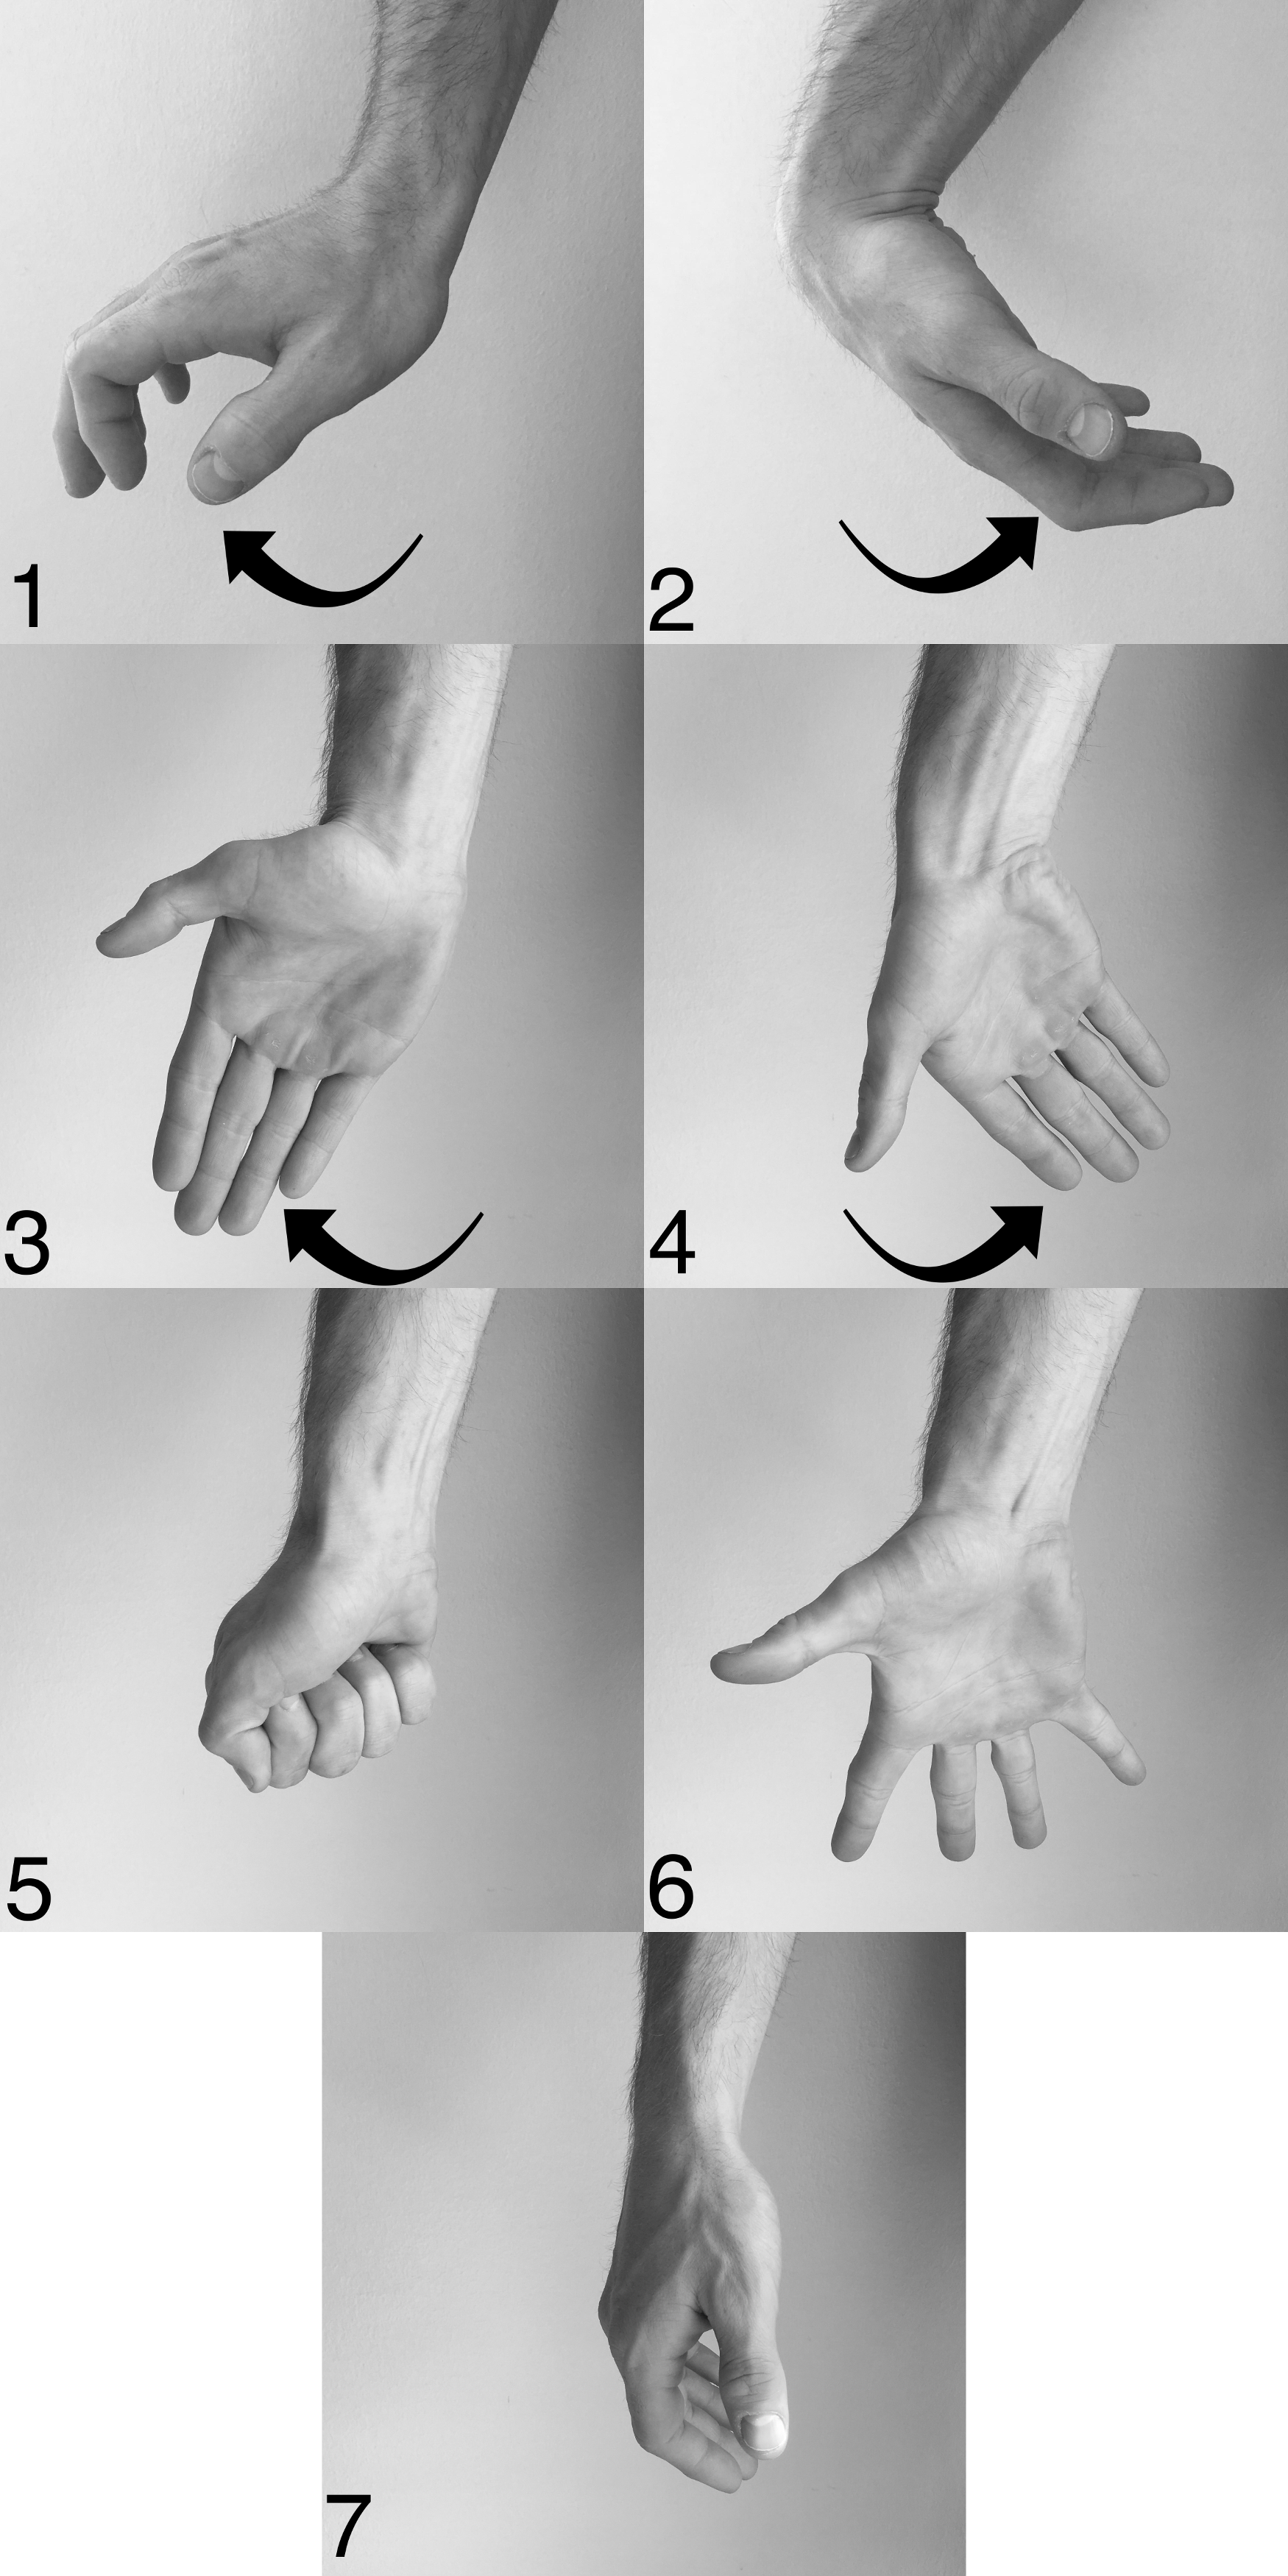
\includegraphics[width=.4\textwidth]{figures/Paper/allHandMovementsVerticalBW}  
	\caption{Illustration of the movements performed in the experiment. 1: Wrist extension, 2: Wrist flexion, 3: Radial deviation, 4: Ulnar deviation, 5: Closed hand, 6: Opened hand, 7: rest.}
	\label{fig:P:experiment_movements} 
\end{figure}

According to Scheme et al. \cite{Scheme2015}, the use of dynamically changing contraction data in training a classification-based control scheme has shown to improve performance and tolerance to proportional control. Based on this finding, the subjects performed three repetitions of each movement, where each repetition constituted of a 2.5 second increasing ramp contraction, a 5 second steady state contraction at the peak of the increasing ramp contraction and a 2.5 second decreasing ramp contraction. To assure that each repetition was carried out correctly, the subjects were instructed in tracking a cursor, representing the EMG signal, on a trapezoidal trajectory, where the slopes corresponded to the ramp contractions and the plateau corresponded to the steady state contraction. The plateau of the trajectory differed between the three repetitions as 40 \%, 50 \% and 70 \% of an initial recorded 15 second constant force of Maximum Voluntary Contraction (MVC). To avoid muscle fatigue the subjects were given 30 seconds rest after an MVC recording and 10 seconds rest between repetitions. 